\chapter{填充颜色}
由于 tikz 绘图默认只能是左对齐,所以可以将它嵌套在表格 table 环
境中,使用表格内容居中,就可以达到中心对齐的目的。
\begin{center}
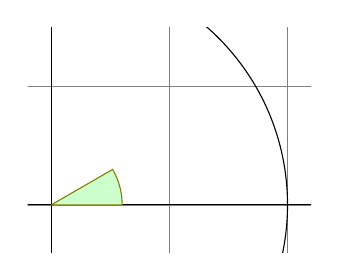
\begin{tikzpicture}[scale=3]%启动绘图环境,并放大 3倍
\clip (-0.1,-0.2) rectangle (1.1,0.75);
\draw[step=0.5cm,gray,very thin] (-1.4,-1.4) grid (1.4,1.4);
\draw (-1.5,0) -- (1.5,0);
\draw (0,-1.5) -- (0,1.5);
\draw (0,0) circle [radius=1cm];
\filldraw[fill=green!20!white,draw=red!50!green] (0,0) -- (3mm,0mm)
arc [start angle=0, end angle=30, radius=3mm] -- (0,0);
\end{tikzpicture}
\end{center}
行间画一段填充扇形。

韦恩图Venn

%韦恩图venn - 两个圆相交
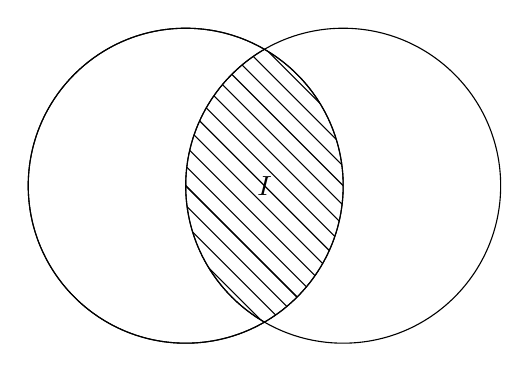
\begin{tikzpicture}
\draw (0,0) circle (2cm);
\draw (2,0) circle (2cm);
\clip[draw] (0,0) circle (2cm);
\clip[draw] (2,0) circle (2cm);
\foreach \x in {-1,-0.75,-0.5,-0.25,0,0,0.25,0.5,0.75,1,1.25,1.5,1.75,2,2.25,2.5,2.75}
\draw[xshift=\x cm]  (-2,2)--(2,-2);
\node at (1,0) {$I$};
\end{tikzpicture}
%韦恩图venn - 3个圆相交
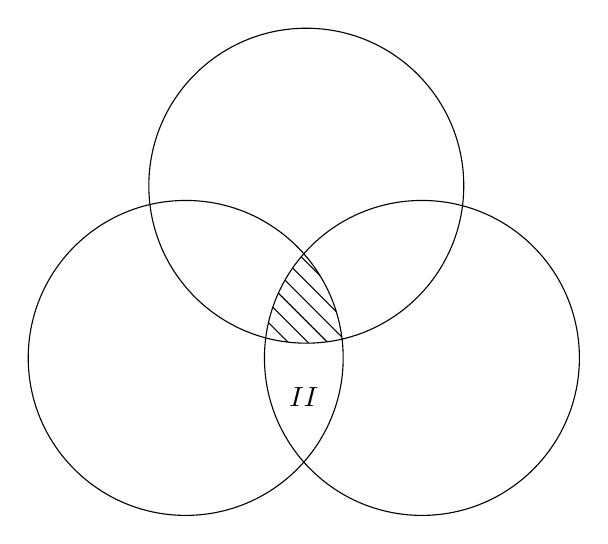
\begin{tikzpicture}
\draw (0,0) circle (2cm);
\draw (55:2.67cm) circle (2cm);
\draw (0:3cm) circle (2cm);
\begin{scope}
\clip (0,0) circle (2cm);
\clip (55:2.67cm) circle (2cm);
\clip (0:3cm) circle (2cm);
\foreach \x in {-1,-0.75,-0.5,-0.25,0,0,0.25,0.5,0.75,1,1.25,1.5,1.75,2,2.25,2.5,2.75}
\draw[xshift=\x cm]  (-2,2)--(2,-2);
\end{scope}
\node at (1.5,-0.5) {$II$};
\end{tikzpicture}

%韦恩图venn - 3个圆相交(斜线填充)
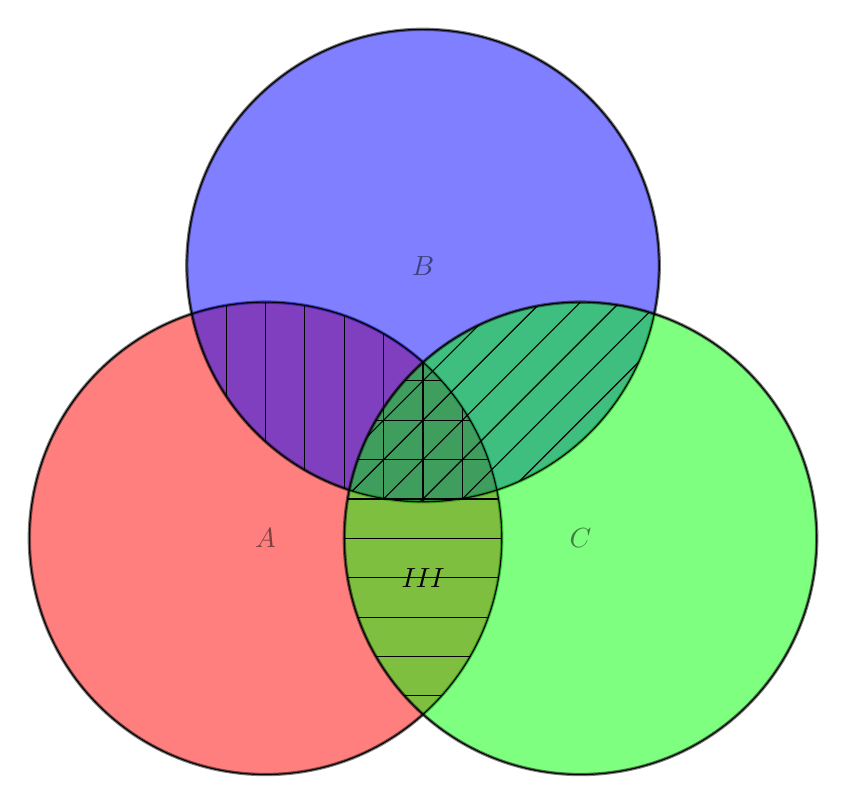
\begin{tikzpicture}  %用[scale=0.8]出问题!
\tikzset{venn circle/.style={draw,circle,minimum width=6cm,fill=#1,opacity=0.5,very thick}}
\node [venn circle = red] (A) at (0,0) {$A$};
\node [venn circle = blue] (B) at (60:4cm) {$B$};
\node [venn circle = green] (C) at (0:4cm) {$C$};
\draw (0,0) circle (3cm);
\draw (60:4cm) circle (3cm);
\draw (0:4cm) circle (3cm);
\begin{scope}
\clip (0,0) circle (3cm);
\clip (60:4cm) circle (3cm);
\foreach \x in {-5,-4.5,-4,-3.5,-3,-2.5,-2,-1.5,-1,-0.5,0,0.5,1,1.5,2,2.5,3,3.5,4,4.5,5}
\draw[overlay, xshift=\x cm]  (2,4)--(2,0);
\end{scope}
\begin{scope}
\clip (60:4cm) circle (3cm);\clip (0:4cm) circle (3cm);
\foreach \y in {-5,-4.5,-4,-3.5,-3,-2.5,-2,-1.5,-1,-0.5,0,0.5,1,1.5,2,2.5,3,3.5,4,4.5,5}
\draw[overlay, xshift=\y cm]  (1,0)--(5,4);
\end{scope}
\begin{scope}
\clip (0,0) circle (3cm);
\clip (0:4cm) circle (3cm);
\foreach \z in {-5,-4.5,-4,-3.5,-3,-2.5,-2,-1.5,-1,-0.5,0,0.5,1,1.5,2,2.5,3,3.5,4,4.5,5}
\draw[overlay, yshift=\z cm]  (0,3)--(4,3);
\end{scope}
\node at (2,-0.5) {$III$};
\end{tikzpicture}

用pattern包填充

\begin{tikzpicture}[red,every node/.style={font=\Large}]
\draw[pattern=north west lines] (0,0) circle(1.5);
\draw (2,0) circle(1.5);
\node[fill=white,inner sep=1pt,rounded corners,below=3] at (90:1.5) {$A$};
\node[xshift=2cm,below=3] at (90:1.5) {$B$};
\end{tikzpicture}

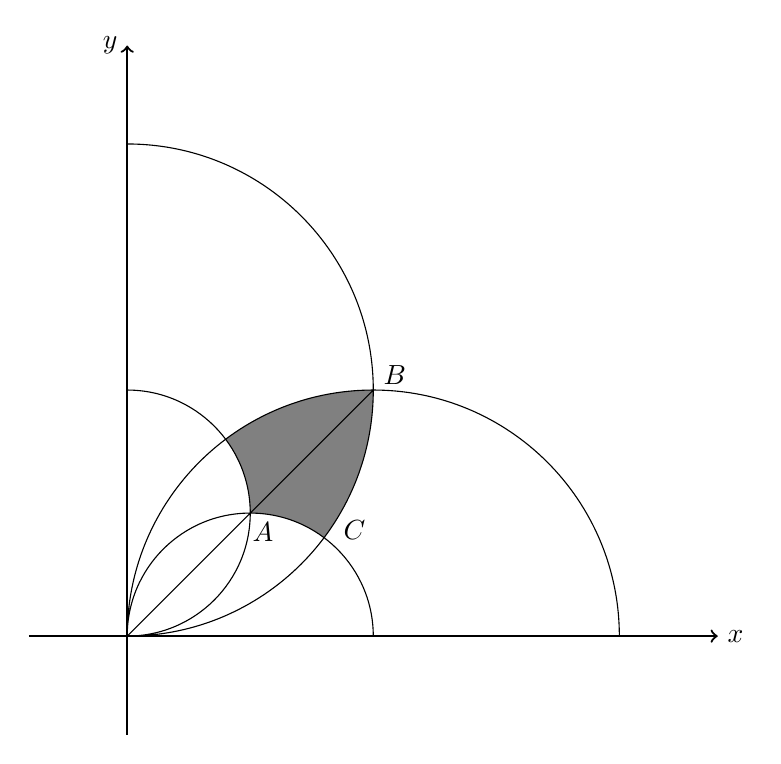
\begin{tikzpicture}[scale=25]
\begin{scope}
\clip (0,0) arc (-90:0:1/8) arc (90:180:1/8);
\fill[gray,even odd rule] (0,0) arc (-90:0:1/8) arc (90:180:1/8)
arc (-90:270:1/16) arc (-180:180:1/16) arc (-90:0:1/16) arc (90:180:1/16);
\end{scope}
\draw [->,thick](-0.05,0)--(0.3,0);\draw [->,thick](0,-0.05)--(0,0.3);
\node[right]at(0.3,0){$x$};\node[left]at(0,0.3){$y$};
\draw (0,0) arc (-90:90:1/8) (0,0) arc (-90:90:1/16)
(0,0) arc (180:0:1/8) (0,0) arc (180:0:1/16) (0,0)--(1/8,1/8);
\node [below]at(0.069,0.0627){$A$};
\node [above]at(0.136,0.123){$B$};
\node [right]at(0.105,0.0541){$C$};
\end{tikzpicture}
\begin{tikzpicture}[scale=25]
\begin{scope}
\clip (0,0) arc (-90:0:1/8) arc (90:180:1/8);
\fill[pattern=horizontal lines]
(0,0) arc (-90:0:1/8) --(1/16,1/16) arc (90:0:1/16);
\fill[pattern=vertical lines]
(0,0) arc (180:90:1/8) --(1/16,1/16) arc (0:90:1/16);
\end{scope}
\draw [->,thick](-0.05,0)--(0.3,0);\draw [->,thick](0,-0.05)--(0,0.3);
\node[right]at(0.3,0){$x$};\node[left]at(0,0.3){$y$};
\draw (0,0) arc (-90:90:1/8) (0,0) arc (-90:90:1/16)
(0,0) arc (180:0:1/8) (0,0) arc (180:0:1/16) (0,0)--(1/8,1/8);
\node [below]at(0.069,0.0627){$A$};
\node [above]at(0.136,0.123){$B$};
\node [right]at(0.105,0.0541){$C$};
\end{tikzpicture}

\begin{tikzpicture}[smooth]
\draw[arrows={-Stealth[length=5pt, inset=3.5pt]}] (-0.5,0) -- (3.0,0)node (xaxis) [right=-1pt] {$x$};
\draw[arrows={-Stealth[length=5pt, inset=3.5pt]}] (0,-0.5) -- (0,4.5)node (yaxis) [above=-0.6pt] {$y$};
\draw  (-0.18,-0.18) node {$o$};
\draw[color=red,domain=0:2.0,fill=green!20] plot (\x,4*\x-\x*\x);
\draw[color=red!40,domain=0:2.90] plot (\x,4*\x-\x*\x)  ;
\draw[color=blue!30,domain=0:2.3] plot (\x,2*\x)  ;
\draw[fill=black] (2,4) circle [radius=0.2pt] node[above=-1.8pt] {$A(2,4)$};
\end{tikzpicture} 
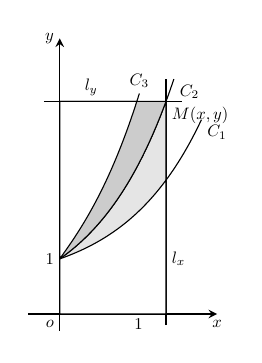
\begin{tikzpicture}[yscale=0.7]
\draw[-stealth] (-0.4,0)--(2,0) node[below,scale=0.6]{$x$};
\draw[-stealth] (0,-0.3)--(0,5) node[left,scale=0.6]{$y$};
\draw (0,0) node [below left,scale=0.6] {$o$};
\foreach \i in {1}{\draw (\i,0)--node [below,scale=0.6] {$1$}(\i,0.05);}
\draw (0,1) node [left,scale=0.6] {$1$};
\draw (1.35,1) node [right,scale=0.6] {$l_x$};
\draw (0.4,3.85742) node [above,scale=0.6] {$l_y$};
\draw (1.35,-0.2) -- (1.35,4.25519);
\draw (-0.2,3.85742) -- (1.55,3.85742);
\draw (1.35,3.85742) node [below right,scale=0.6] {$M(x,y)$};
%\clip (-1,-1) rectangle (5,5);%只在这个区域内画图
\draw[domain=1:4,smooth,variable=\t] plot ({ln(\t)+1/(2*\t)-0.5},\t)node[above,scale=0.6] {$C_3$};
\draw[domain=0:1.8,smooth] plot (\x,{0.5*1+0.5*exp(\x)}) node[below right,scale=0.6] {$C_1$};
\draw[domain=0:1.45,smooth] plot (\x,{exp(\x)}) node[below right,scale=0.6] {$C_2$};
\filldraw [fill=gray!20] (0,0) -- plot [domain=0:1.35,smooth] (\x,{exp(\x)}) -- (1.35,0) -- (0,0);
\filldraw [fill=white] (0,0) -- plot [domain=0:1.35,smooth] (\x,{0.5*1+0.5*exp(\x)}) -- (1.35,0) -- (0,0);
\filldraw [fill=gray!40] (0,1) -- plot [domain=0:1.35,smooth] (\x,{exp(\x)}) -- (0,3.85742) -- (0,1);
\filldraw [fill=white] (0,1) -- plot [domain=1:3.85742,smooth,variable=\t] ({ln(\t)+1/(2*\t)-0.5},\t) -- (0,3.85742) -- (0,1);
\end{tikzpicture}

\begin{tikzpicture}[scale=1.5]
\draw[-stealth] (-0.3,0) -- (2.2,0)node (xaxis) [right,scale=0.8] {$x$};
\draw[-stealth] (0,-1.6) -- (0,1.6)node (yaxis) [left,scale=0.8] {$y$};
\fill[pink!] (0,0) -- (1,-1) arc [start angle=315, end angle=405, radius=1.414] -- (0,0);
\fill[pink!] (1,0) -- (1,1) arc [start angle=90, end angle=180, radius=1] -- (0,0);
\fill[grassgreen] (0,0) -- (1,-1) arc [start angle=315, end angle=360, radius=1.414] -- (1.414,0)--(2,0) arc [start angle=360, end angle=270, radius=1] -- (1,-1);
\fill[grassgreen] (0,0) -- (1,1) arc [start angle=45, end angle=0, radius=1.414] -- (1.414,0)--(2,0) arc [start angle=0, end angle=90, radius=1] -- (1,1);
\draw (1,-0.02)--(1,0.02) node[below] {$\scaleobj{0.6}{1}$};
\draw (1.414,-0.02)--(1.414,0.02) node[below] {$\scaleobj{0.6}{\sqrt{2}}$};
\draw[style=dashed,color=red,domain=-0.1:1.4] plot(\x,-\x);
\draw[color=black,domain=-0.1:2.2] plot(\x,0);
\draw[style=dashed] (0,0)--(0,-1.414) arc [start angle=270, end angle=450, radius=1.414];
\draw (1,0) circle [radius=1];
%\fill[pattern=north west lines](0,0)--(-2,0)--(-2,2)--(0,2)arc(90:270:0.8);
%\fill[pattern=north west lines]arc(-45:0:1);
\end{tikzpicture}
\section{填充}
画一个带渐变阴影的形状。默认阴影是从灰到白。 当然你可以设置不同颜色及不同的渐变方式, 比如中心渐变,左部渐变等。

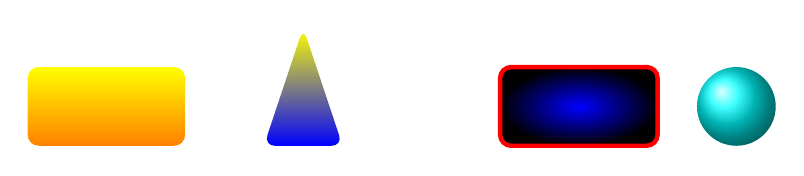
\begin{tikzpicture}[rounded corners, ultra thick]
\shade [top color=yellow, bottom color=orange] (0,0) rectangle +(2,1);
\shade [top color=yellow, bottom color=blue] (3,0) -- (4,0) -- (3.5 ,1.5) -- cycle;
\shadedraw [inner color=blue, outer color=black, draw = red] (6,0) rectangle +(2,1);
\shade[ball color=cyan] (9, 0.5) circle (0.5cm);
\end{tikzpicture}

用法:
\begin{verbatim}
\fill[options] (x1,y1) -- (x2,y2) arc (angle1:angle2:radius) -- (x3,y3);
\fill[options] (x1,y1) -- (x2,y2) arc (angle1:angle2:radius) -- cycle; % better
\filldraw[options] (x1,y1) -- (x2,y2) arc (angle1:angle2:radius) -- cycle;
\end{verbatim}
\begin{lstlisting}
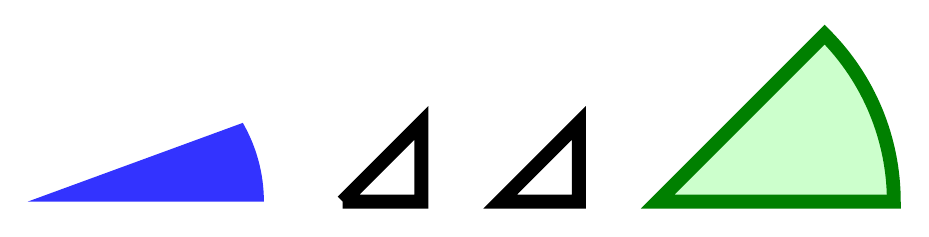
\begin{tikzpicture}[line width=5pt]
\fill[blue!80] (0,0) -- (3,0) arc (0:30:2) -- (0,0);
\draw (4,0) -- (5,0) -- (5,1) -- (4,0);
\draw (6,0) -- (7,0) -- (7,1) -- cycle;
\filldraw[fill=green!20!white, draw=green!50!black]
(8,0) -- (11,0) arc (0:45:3) -- cycle;
\end{tikzpicture}
\end{lstlisting}
\begin{center}
	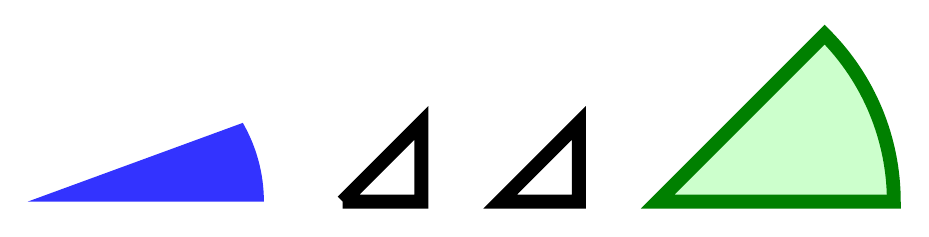
\begin{tikzpicture}[line width=5pt]
	\fill[blue!80] (0,0) -- (3,0) arc (0:30:2) -- (0,0);
	\draw (4,0) -- (5,0) -- (5,1) -- (4,0);
	\draw (6,0) -- (7,0) -- (7,1) -- cycle;
	\filldraw[fill=green!20!white, draw=green!50!black]
	(8,0) -- (11,0) arc (0:45:3) -- cycle;
	\end{tikzpicture}
\end{center}

\section{阴影}
用法:
\begin{verbatim}
\shade[options] (x1,y1) rectangle (x2,y2);
\shadedraw[options] (x1,y1) circle (radius);
\end{verbatim}
\begin{lstlisting}

\begin{tikzpicture}[rounded corners,ultra thick]
\shade (0,0) rectangle (2,1);
\shadedraw (3,0.5) circle (.5cm);
\shade[top color=yellow,bottom color=black] (0,0) rectangle +(2,1);
\shade[left color=yellow,right color=black] (3,0) rectangle +(2,1);
\shadedraw[inner color=yellow,outer color=black,draw=yellow] 
(6,0) rectangle +(2,1);
\shade[ball color=green] (9,.5) circle (.5cm);
\shadedraw[left color=gray,right color=green, draw=green!50!black]
(10,0.3) -- +(1,0) arc (0:30:1) -- cycle;
\end{tikzpicture}
\end{lstlisting}

\begin{tikzpicture}[rounded corners,ultra thick]
\shade (0,0) rectangle (2,1);
\shadedraw (3,0.5) circle (.5cm);
\shade[top color=yellow,bottom color=black] (0,0) rectangle +(2,1);
\shade[left color=yellow,right color=black] (3,0) rectangle +(2,1);
\shadedraw[inner color=yellow,outer color=black,draw=yellow] 
(6,0) rectangle +(2,1);
\shade[ball color=green] (9,.5) circle (.5cm);
\shadedraw[left color=gray,right color=green, draw=green!50!black]
(10,0.3) -- +(1,0) arc (0:30:1) -- cycle;
\end{tikzpicture}